\section{Types of Periodograms}

The following will look at ``Welch'' and ``Lomb-Scargle'' periodograms and some python implementations with \inlinecodee{numpy} and \inlinecodee{scipy}.\\

Two test signals, $A$ and $B$, are defined for this purpose:
\[
  A(t) = 1\,\si{\volt}\sin{(2\pi \cdot {\color{red-5}100.5}\,\si{\hertz}\cdot t) + 0.6\,\si{\volt}\cdot\sin{(2\pi\cdot {\color{red-5}199.5}\,\si{\hertz}\cdot t)}}
\]

\[
  B(t) = 1\,\si{\volt}\sin{(2\pi \cdot {\color{red-5}{100.5}}\,\si{\hertz}\cdot t) + 0.6\,\si{\volt}\cdot\sin{(2\pi\cdot {\color{red-5}{109.5}}\,\si{\hertz}\cdot t)}}
\]

Gaussian noise with a standard deviation of $\sigma=1\,\si{\volt}$ is added to each of these signals and their standard periodograms will be compared with the Welch and Lomb-Scargle periodograms.

\subsection{Welch Periodograms}
Welch's method is a modified type of periodogram. Instead of transforming the whole input sequence into the frequency domain, the sequence is split into multiple overlapping\footnote{without overlapping, this method is called ``Bartlett's Method''} intervals (windowed). Then, all the individual power spectra of these intervals are calculated and averaged to produce the final periodogram. The overlapping of the segments can help to restore some of the power content on the edges of the segments that was lost due to windowing. Figure \ref{fig:welch_ill} shows an illustration of this method.\\

\begin{figure}[h]
\centering
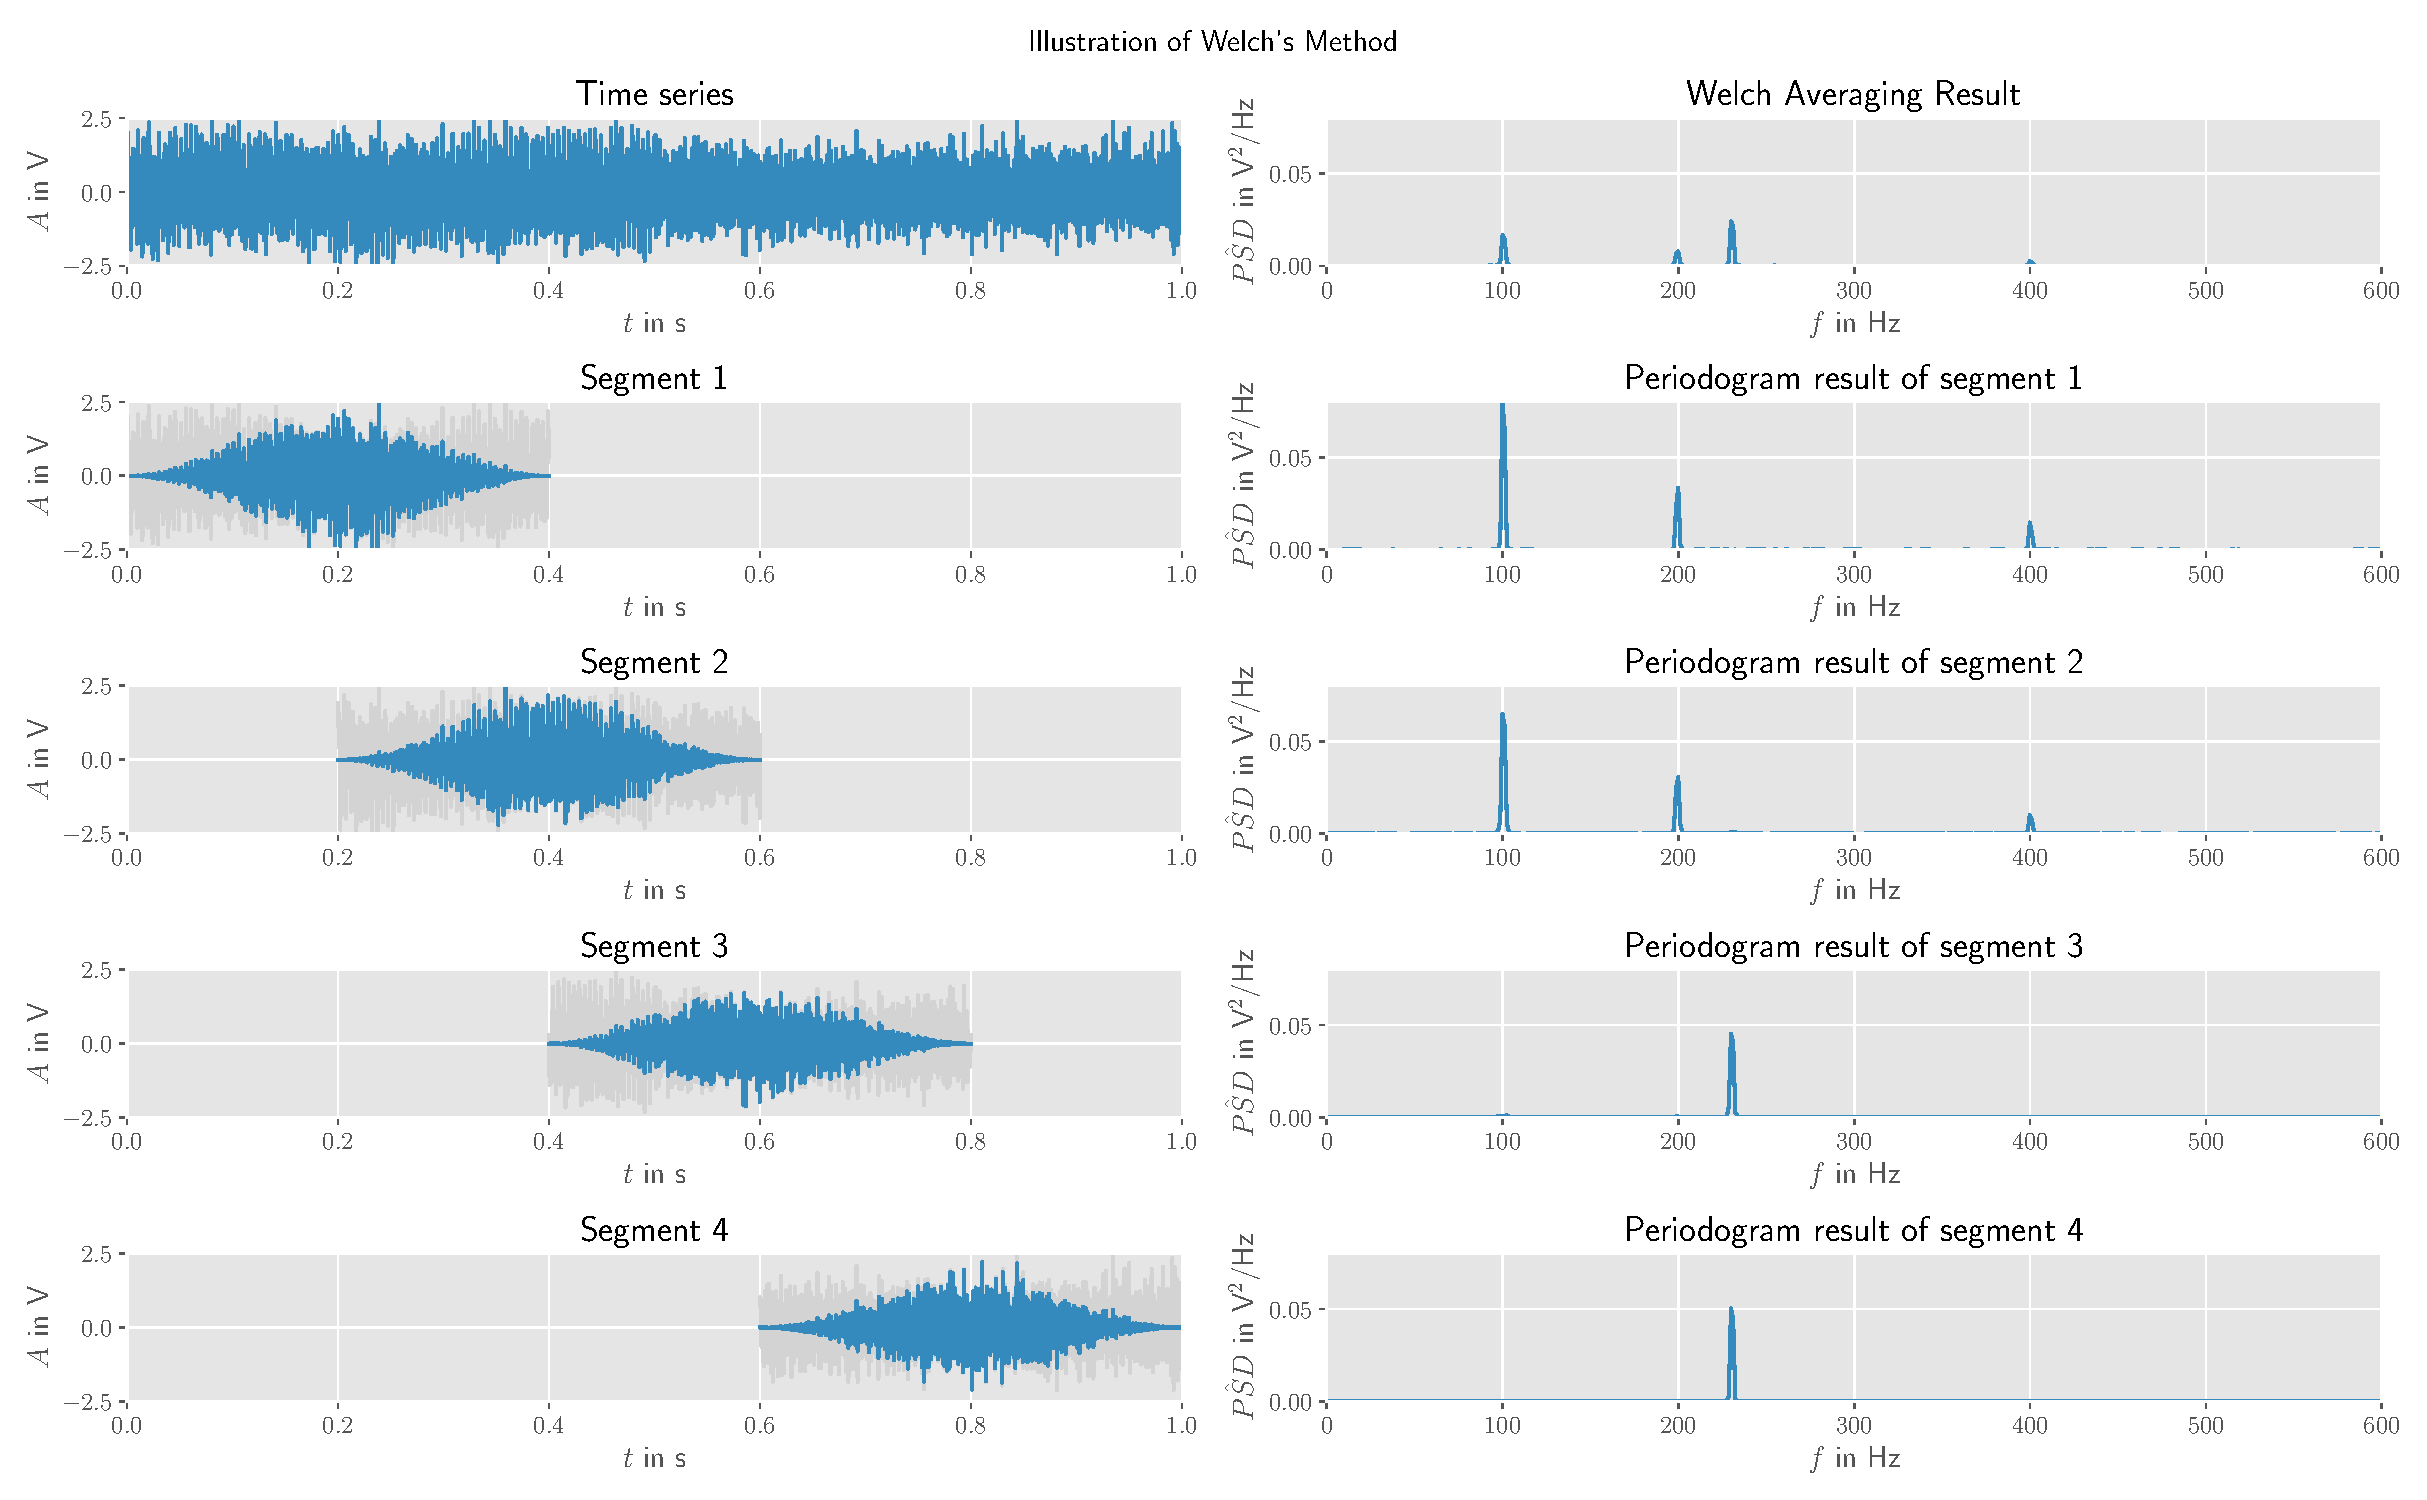
\includegraphics[width=\textwidth]{graphics/welch_illustration.pdf}
\caption{Illustration of Welch's method. The time series is split into multiple windowed segments which are then individually transformed into periodograms that are averaged to obtain the overall periodogram. In this case, the 4 segments were windowed with a Hann window. The total size is $N= 6000$.}\label{fig:welch_ill}
\end{figure}

Due to the averaging approach of Welch's method, the resulting periodogram might be less sensitive to noise in the time series. E.g. think about a short-duration noise spike in the data: In the full FFT, it might introduce large high frequency content but in the Welch periodogram it will only be evaluated in a fraction of the segments and therefore might not be visible after averaging.\\

However, since the splitting of the sequence into segments reduces the time window of each individual FFT, the frequency resolution will be smaller than the FFT of the whole sequence ($\frac{1}{T_{w}}$).
This can become a problem when trying to distinguish harmonics of the signal that are relatively closely spaced in frequency.\\

Adjustable parameters of this method include the segment size, the overlapping size, and the window applied.

Figure \ref{fig:welch_exp} shows the periodograms of both test signals and compares them to the standard periodogram. The noise level has been reduced by the Welch periodogram. However, the frequencies of signal $B$ are not distinguishable anymore due to the reduced frequency resolution. The code for this can be found in appendix \ref{app:welch}. Figure \ref{fig:welch_comp} further shows that the application of the Welch window requires a tradeoff of its parameters.

\begin{figure}[h]
\centering
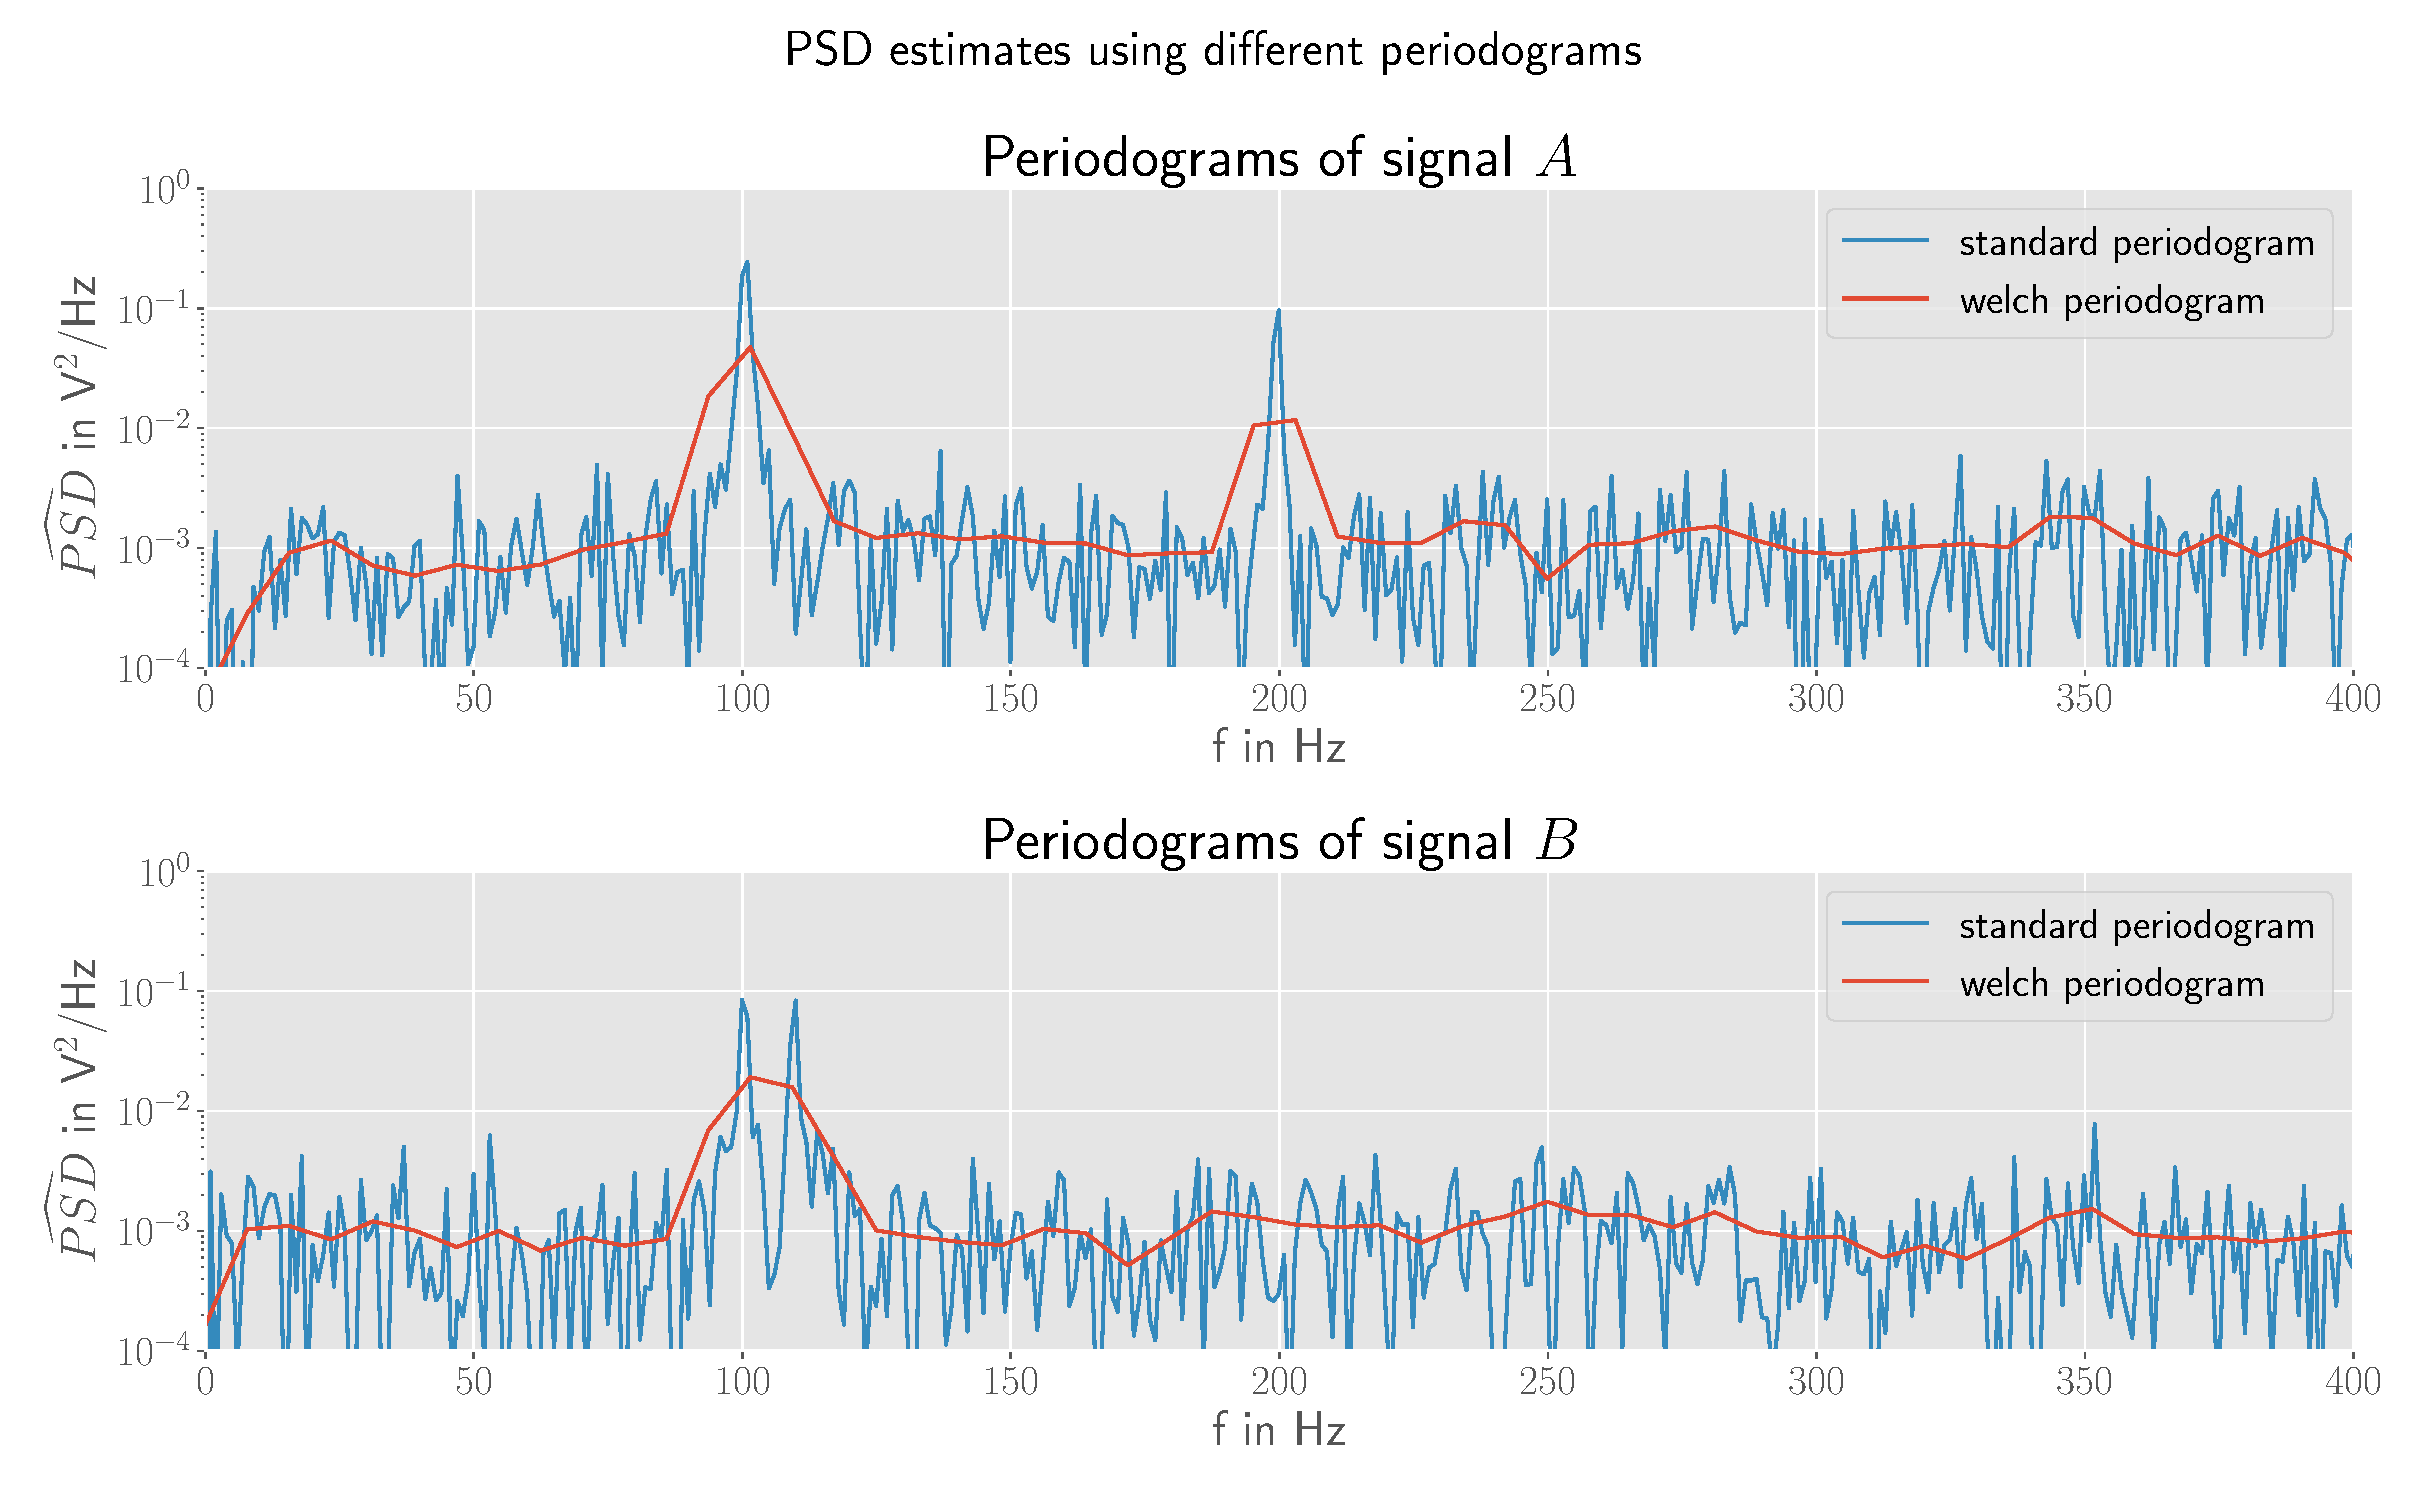
\includegraphics[width=0.764\textwidth]{graphics/welch.pdf}
\caption{Comparison of standard and welch periodograms. \inlinecodee{scipy}'s default parameters have been used for the Welch periodograms.}\label{fig:welch_exp}
\end{figure}


\begin{figure}[H]
\centering
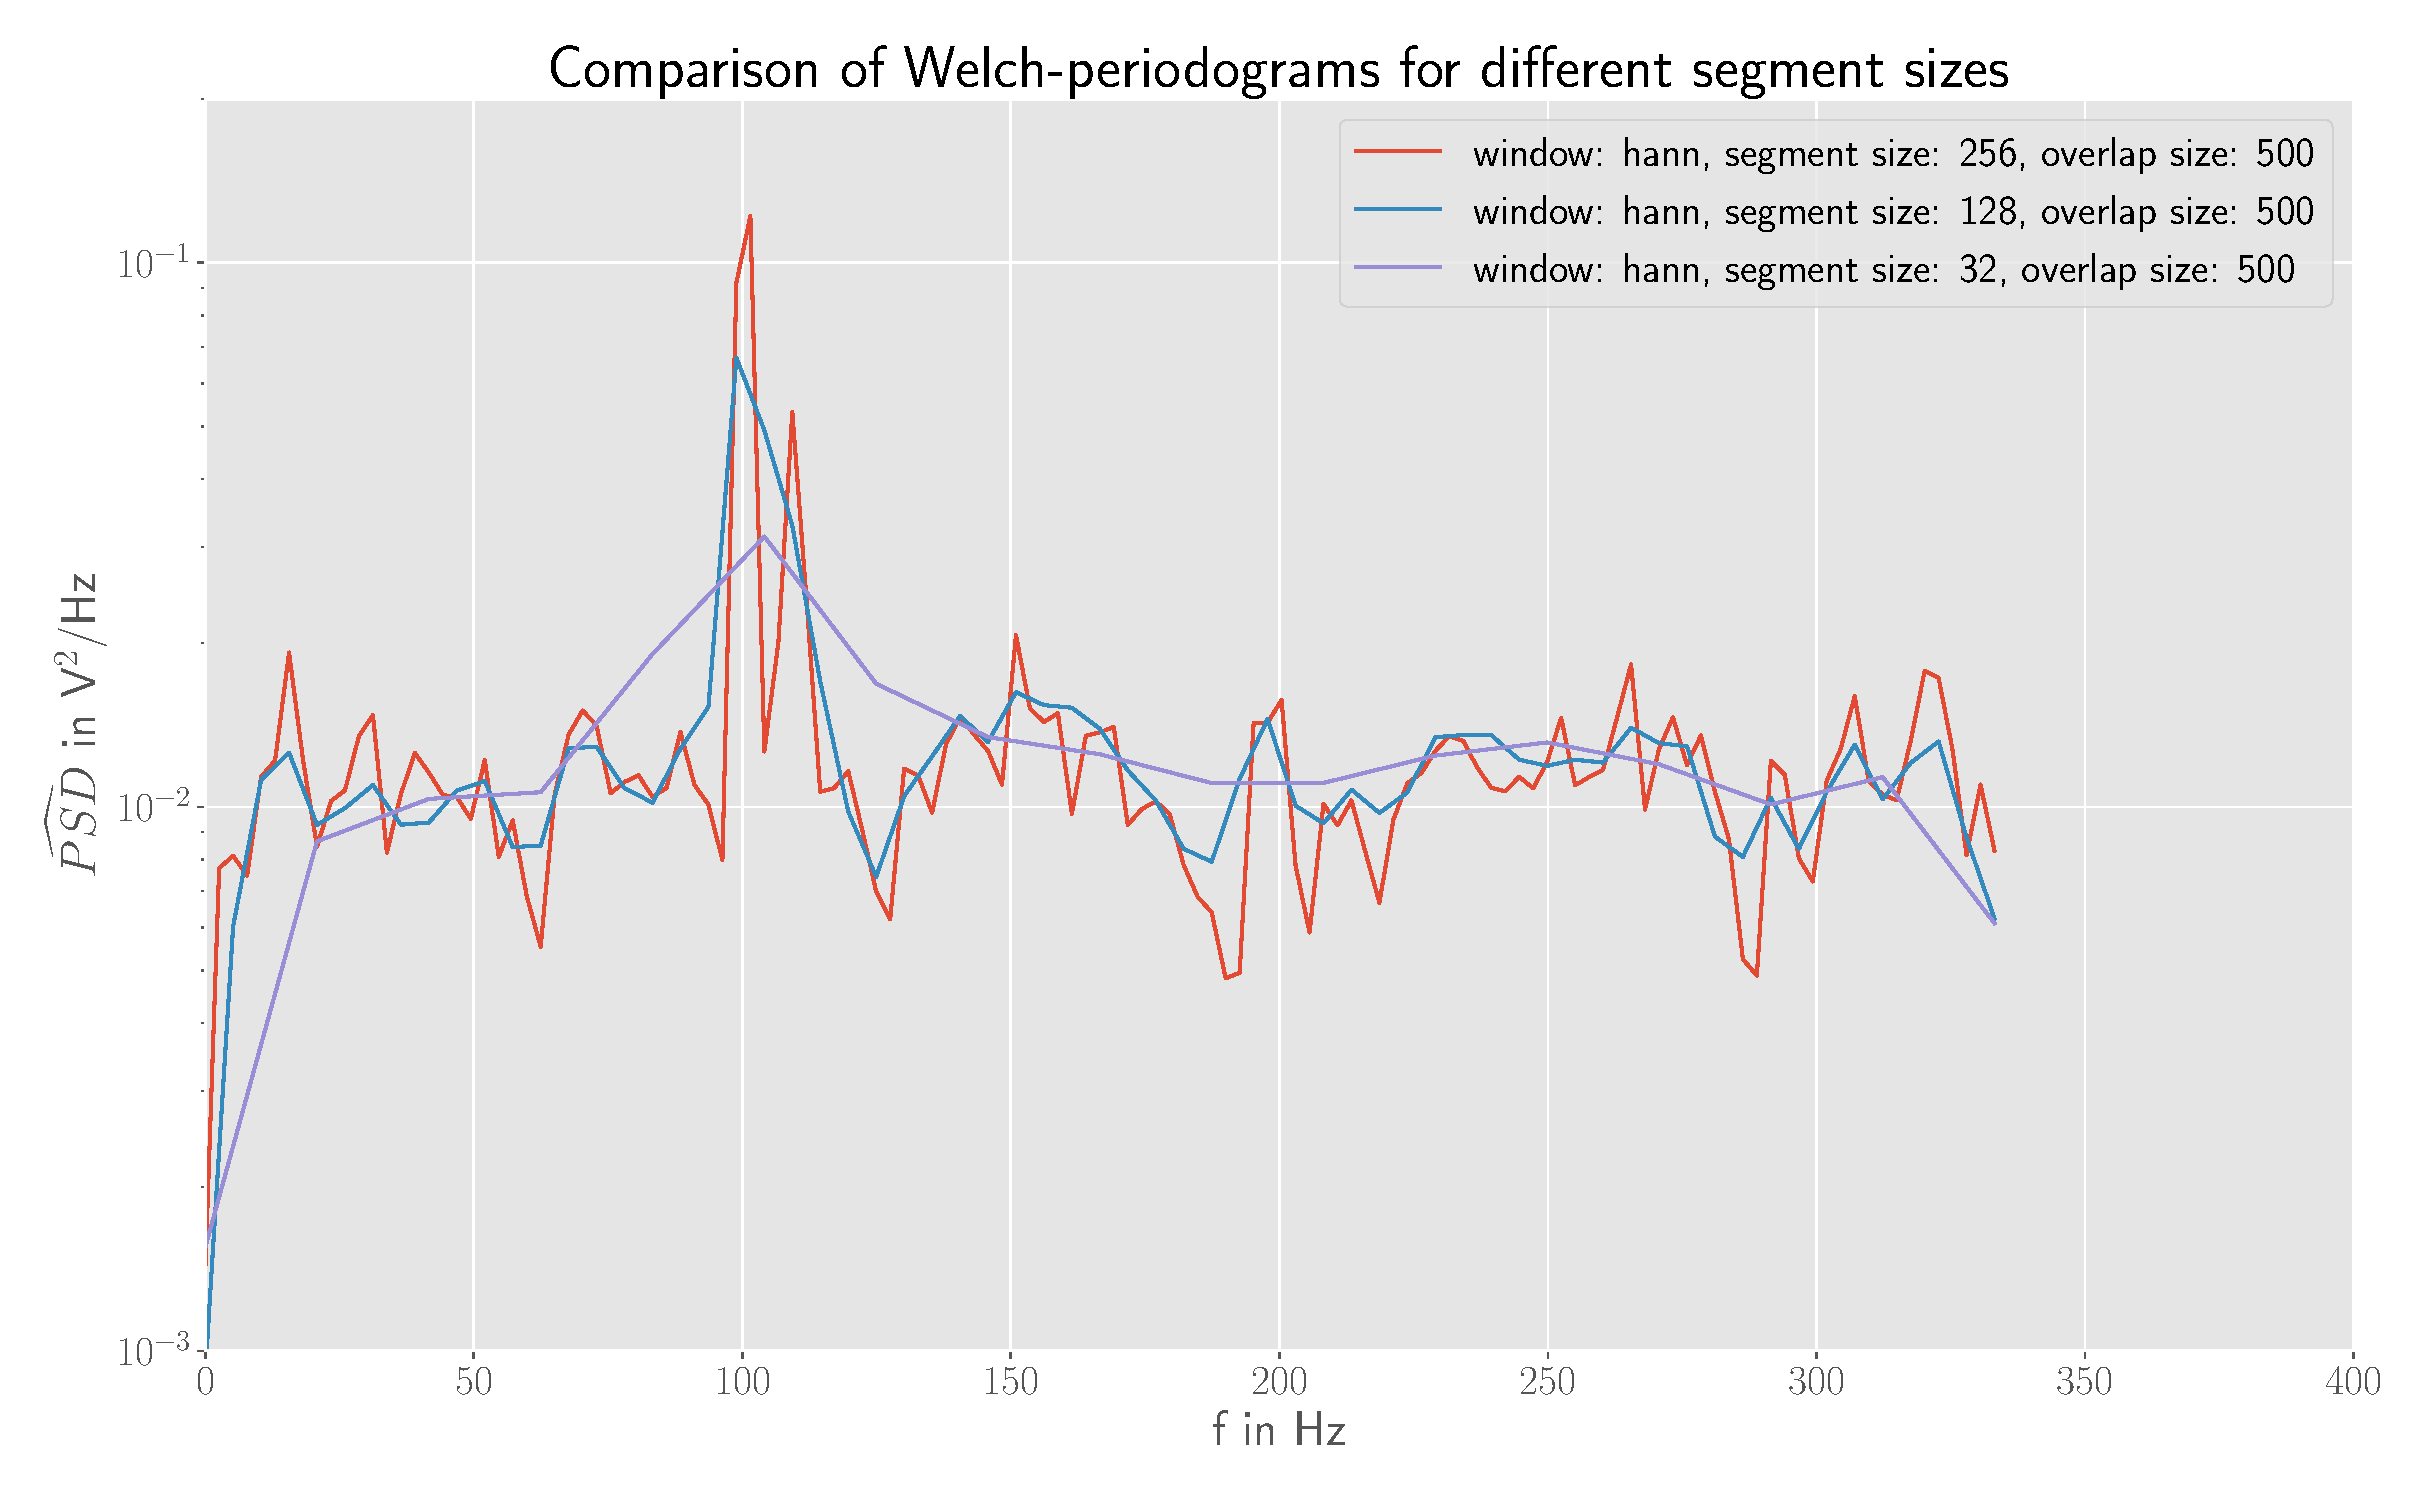
\includegraphics[width=0.764\textwidth]{graphics/welch_comp.pdf}
\caption{Comparison of different Welch segment sizes when applied to signal $B$. For code see appendix \ref{app:welch_comp}.}\label{fig:welch_comp}
\end{figure}


\subsection{Lomb-Scargle Periodograms}
The \textit{Lomb-Scargle} method of PSD-estimation can be classified as a method of ``Least-squares spectral analysis'' (LSSA). LSSA tries to extend the periodogram estimation to data sequences that are not necessarily sampled in an equally-spaced manner. This also applies if individual samples of the data are lost or could not be aquired and will remove the need to resample or interpolate the data. \cite{lomb_1}\cite{yt_video}\\

Instead of explicitly performing the Fourier transform, the Lomb-Scargle periodogram estimates the PSD using a sinusoidal model that matches the data. The Lomb-Scargle technique looks for the model that best explains the data as a sum of sinusoids with various frequencies and amplitudes.

The algorithm first determines a range of frequencies for measuring the PSD. These frequencies, which might be evenly or logarithmically separated, are determined by the frequency range anticipated in the signal. The program then uses a weighted sum of the data points, where the weights vary depending on how well the model fits the data, to compute a power estimate at each frequency.

Least-squares fitting is employed to determine the weights. In order to achieve this, one must identify the set of parameters that minimizes the total of the squared discrepancies between the model and the data at each moment. These weights are then used by the algorithm to determine the power estimate for each frequency.

However, the method has significant drawbacks. It's assumption that the signal is stationary, which may not be the case for all signal types, is one of its limitations. The method may also be sensitive to the selection of model parameters, such as the quantity of frequencies employed in the model or the frequency range assessed. \cite{saqib_1}\cite{saqib_2}\cite{saqib_3}\\

To simulate this method, signal $A$ was sampled at uniformly distributed random times. As seen in Figure \ref{fig:lomb_1}, the Lomb-Scargle periodogram approximately follows the standard periodogram.


\begin{figure}[H]
\centering
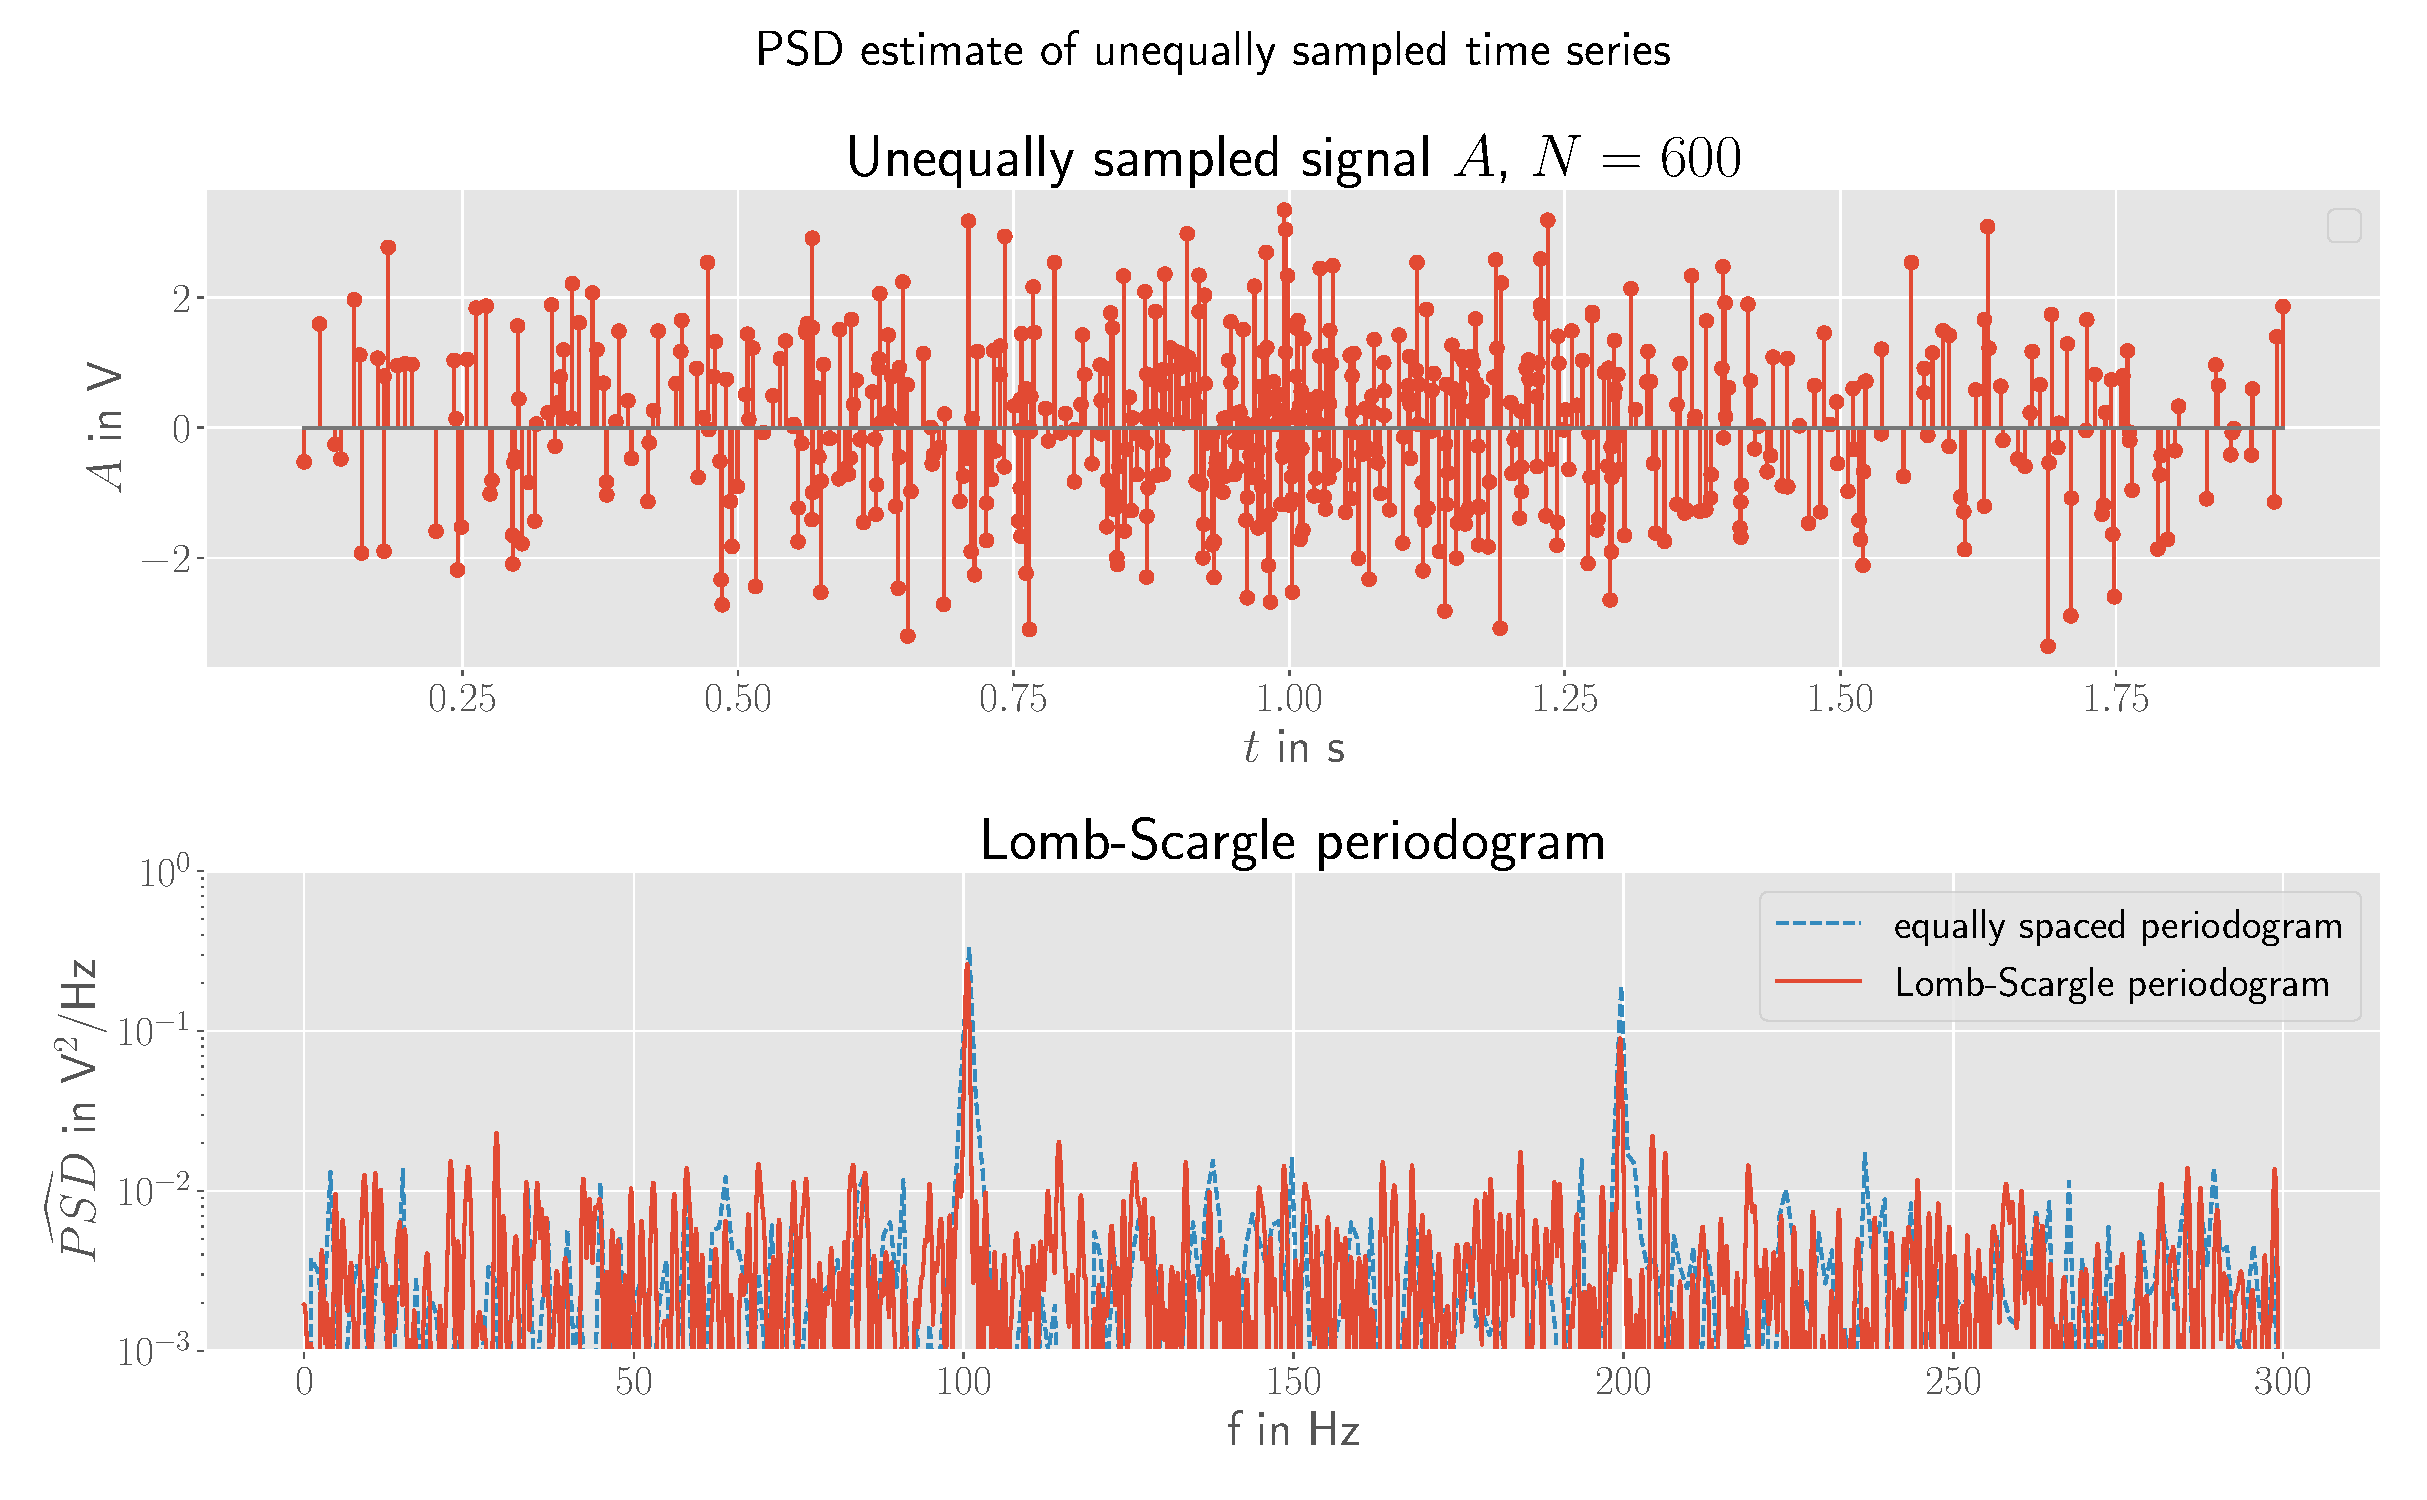
\includegraphics[width=0.764\textwidth]{graphics/lomb_scargle.pdf}
\caption{Lomb-Scargle PSD estimate of an unevenly spaced }\label{fig:lomb_1}
\end{figure}


